\documentclass[tikz]{standalone}
\usetikzlibrary{hobby, arrows.meta,bending,decorations.markings}
\begin{document}
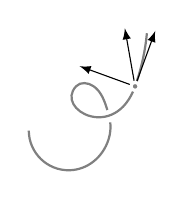
\begin{tikzpicture}[baseline,scale=.75]
\draw[gray,thick] (.1,.85) to [curve through={(.79,.18) .. (1.45,.7) (1.48,.99) .. ([blank=soft]1.43,1.2) .. (1.2,1.6) .. (.9,1.6) .. (1.9,1.6)}] (2.1,2.5);
%\draw[thick,-stealth] (1.9,1.6) -- ({1.9+cos(20)},{1.6+sin(20)});
%\draw[thick,-stealth] (1.9,1.6) -- ({1.9+cos(50)},{1.6+sin(50)});
%\draw[thick,-stealth] (1.9,1.6) -- ({1.9+cos(110)},{1.6+sin(110)});
\draw[-latex] (1.9,1.6) -- ({1.9+cos(70)},{1.6+sin(70)});
\draw[-latex] (1.9,1.6) -- ({1.9+cos(100)},{1.6+sin(100)});
\draw[-latex] (1.9,1.6) -- ({1.9+cos(160)},{1.6+sin(160)});
\fill[gray,draw=white,very thick] (1.9,1.6) circle (2pt);
\end{tikzpicture}
\end{document}
